\documentclass[xcolor={usenames,dvipsnames,svgnames,table}]{beamer}
\usepackage{beamer_rwth_theme}
\usepackage{ulem}
\newcommand{\av}[1]{\ensuremath{\langle #1 \rangle}\xspace}

\begin{document}

%----------------------------------------------------------------

% taken from
% http://www.lns.cornell.edu/~pt267/files/code/TikZFeynman.tex

%\usepackage{tikz}
\usetikzlibrary{arrows,shapes}
\usetikzlibrary{trees}
\usetikzlibrary{matrix,arrows} 				% For commutative diagram
											% http://www.felixl.de/commu.pdf
\usetikzlibrary{positioning}				% For "above of=" commands
\usetikzlibrary{calc,through}				% For coordinates
\usetikzlibrary{decorations.pathreplacing}  % For curly braces
% http://www.math.ucla.edu/~getreuer/tikz.html
%\usepackage{pgffor}							% For repeating patterns

\usetikzlibrary{decorations.pathmorphing}	% For Feynman Diagrams
\usetikzlibrary{decorations.markings}
\tikzset{
	>=stealth', %%  Uncomment for more conventional arrows
    vector/.style={decorate, decoration={snake}, draw},
	provector/.style={decorate, decoration={snake,amplitude=2.5pt}, draw},
	antivector/.style={decorate, decoration={snake,amplitude=-2.5pt}, draw},
    fermion/.style={draw=black, postaction={decorate},
        decoration={markings,mark=at position .55 with {\arrow{>}}}},
    fermionbar/.style={draw=black, postaction={decorate},
        decoration={markings,mark=at position .55 with {\arrow{<}}}},
    fermionnoarrow/.style={draw=black},
    gluon/.style={decorate, draw=black,
        decoration={coil,amplitude=4pt, segment length=5pt}},
    scalar/.style={dashed,draw=black, postaction={decorate},
        decoration={markings,mark=at position .55 with {\arrow{>}}}},
    scalarbar/.style={dashed,draw=black, postaction={decorate},
        decoration={markings,mark=at position .55 with {\arrow{<}}}},
    scalarnoarrow/.style={dashed,draw=black},
    electron/.style={draw=black, postaction={decorate},
        decoration={markings,mark=at position .55 with {\arrow{>}}}},
	bigvector/.style={decorate, decoration={snake,amplitude=4pt}, draw},
}

\def\tikzoverlay{%
 \tikz[baseline,overlay]\node[every overlay node]
}%


%----------------------------------------------------------------------------------------
%	TITLE PAGE
%----------------------------------------------------------------------------------------

\title{\huge{New Results on Particle and Astroparticle Physics with an Emphasis on Higgs Physics}}
\author{Peter Fackeldey}
\vspace*{-.7cm}
\date{\today}

\begin{frame}[noframenumbering,plain]
 \titlepage
\end{frame}

% ===========================================================
% Slides
% ===========================================================
\begin{frame}
	\frametitle{O Higgs Boson, where art thou?}
	\centering \textcolor{color1}{Preparation time: 1964 - 2008}
	\begin{tabbing}
		\hspace{1cm}\=\hspace{1cm}\=\kill
		\> 400\'{} ml \> Theorists! (Brout, Englert, Higgs and GHK) \\
		\> 800\'{} g \> New theory: Higgs mechanism\\
		\> 3\'{} cups\> 1964 Symmetry breaking papers\\
		\> 1\'{} tbsp \> Circular collider (LHC)\\
		\> 1\'{} cup \> Detector (CMS/ATLAS)\\
	\end{tabbing}
	\centering \textcolor{color1}{Cooking time: 2009 - 2012}
	\begin{tabbing}
		\hspace{1cm}\=\hspace{1cm}\=\kill
		\> 2\'{} tsp \> Proton bunches\\
		\> 10\'{} oz \> Grid computing (CERN, FNAL, KIT, ...)\\
		\> 5\'{} g \> Analysis software \\
		\> 1000\'{} cans \> Low-paid grad students\\
	\end{tabbing}
\end{frame}

\begin{frame}
    \frametitle{Higgs Mechanism: A New Hope}
    \begin{itemize}
        \item \underline{\textbf{Problem:}} The Standard Model (SM) misses mass terms for the weak gauge bosons
        \item \underline{\textbf{Proposal:}} Spontaneous electroweak symmetry breaking (Higgs mechanism)
        \item New scalar field $\Phi$ based on the following lagrangian is introduced:
    \end{itemize}
    \begin{gather*}
        \label{eq_lagrangian_higgs}
        \mathcal{L}_\mathrm{Higgs} = \underbrace{(\mathrm{D}\xspace^\mu \, \Phi)^\dagger (\mathrm{D}\xspace_\mu \, \Phi)}_{\text{\textcolor{color2}{Kinetic}}} \underbrace{- \mu^2 \, \Phi^\dagger \, \Phi - \lambda {(\Phi^\dagger \, \Phi})^2}_{\text{\textcolor{color2}{Potential}}} \quad \text{with} \quad \Phi =  \begin{pmatrix} \phi^+ \\ \phi^0 \end{pmatrix}
    \end{gather*}
    \begin{itemize}
        \item \textcolor{color2}{Potential} contains two terms:
        \begin{itemize}
            \item Mass term: $- \mu^2 \, \Phi^\dagger \, \Phi $: $\mu^2$ can be negative or positive
            \item Self-coupling term: $- \lambda (\Phi^\dagger \, \Phi)^2$: $\lambda$ is a dimensionless positive constant
        \end{itemize}
    \end{itemize}
\end{frame}

\begin{frame}
    \frametitle{Revenge of the Symmetry Breaking}
    \begin{itemize}
        \item \sout{If $\mu^2>0$ there is only one ground state possible: $\av{\Phi}_0=0$}
        \item If $\mu^2<0$ there are multiple ground states:
    \end{itemize}
    \begin{gather*}
        \abs{\av{\Phi}_0}^2 = -\frac{\mu^2}{2 \, \lambda} \equiv \frac{v^2}{2} \quad \text{with} \quad v=\text{vacuum expectation value}
    \end{gather*}
    \begin{itemize}
        \item In a general way without the loss of $\mathrm{SU}(2)$ invariance:
    \end{itemize}
    \begin{gather*}
        \av{\Phi}_0 = \frac{1}{\sqrt 2} \, \begin{pmatrix} 0 \\ v \end{pmatrix} \quad \Rightarrow \quad \Phi(x) = \frac{1}{\sqrt 2} \, \begin{pmatrix} 0 \\ v + H(x) \end{pmatrix}
    \end{gather*}
    \begin{itemize}
        \item $H(x)$ describes the Higgs field
    \end{itemize}
\end{frame}

\begin{frame}
    \frametitle{The Mass Terms Awakens}
    \begin{itemize}
        \item Kinetic term $\abs{\mathrm{D}\xspace_\mu \, \Phi}^2$:
    \end{itemize}
    \begin{align*}
        %\abs{\covdif_\mu \, \Phi}^2 = \frac 1 2 \del{\partial_\mu \, H}^2 + \frac 1 8 \, g_2^2 \del{v+H}^2 \, \abs{W_\mu^1 + \im \, W_\mu^2}^2 + \frac 1 8 \del{v+H}^2 \, \abs{g_2 \, W_\mu^3 - g_1 \, B_\mu}^2
        \abs{\mathrm{D}\xspace_\mu \, \Phi}^2 &= \frac 1 8 \, v^2 \, g_2^2 \, \abs{W_\mu^1 + \im \, W_\mu^2}^2 + \frac 1 8 \, v^2 \, \abs{g_2 \, W_\mu^3 - g_1 \, B_\mu}^2 + \, \ldots \\
        &= \frac 1 2 \, \textcolor{color2}{m_W}^2 \, W_\mu^+ \, W^{- \mu} + \frac 1 2 \, \textcolor{color2}{m_Z}^2 \, Z_\mu \, Z^\mu + \, \ldots
    \end{align*}
    \begin{itemize}
        \item \textcolor{color2}{Mass} terms occur for the weak gauge bosons!
        \item Potential of the lagrangian $V(x)$:
    \end{itemize}
    \begin{gather*}
        V = \frac 1 2 \, \mu^2 \, (v+H)^2 + \frac 1 4 \, \lambda (v+H)^4 \quad \Rightarrow \quad \textcolor{color2}{m_H} = -\sqrt 2 \, \mu = v \, \sqrt{2 \, \lambda}
    \end{gather*}
    \begin{itemize}
        \item \textcolor{color2}{Mass} term for the Higgs Boson, the excitation of $H(x)$, occurs
    \end{itemize}
\end{frame}

\begin{frame}
    \frametitle{The Yukawa Interaction Strikes Back}
    \begin{itemize}
        \item The fermion masses can not be described by the Higgs mechanism, due to the chirality
        \item An interaction between \textcolor{color1}{Dirac (fermion) fields} and a \textcolor{color2}{scalar (Higgs) field} is described by Yukawa interaction:
    \end{itemize}
    \begin{gather*}
        \label{eq_lagrangian_yukawa}
        \mathcal{L}_\mathrm{Yukawa} = - \lambda_f \, \textcolor{color1}{\ensuremath{\psi}\xspace_\mathrm{L}^\dagger} \, \textcolor{color2}{\Phi} \, \textcolor{color1}{\ensuremath{\psi}\xspace_\mathrm{R}}
    \end{gather*}
    \begin{itemize}
        \item Lagrangian for fermion mass:
    \end{itemize}
    \begin{gather*}
        \label{eq_lagrandian_mf}
        \mathcal{L}_\mathrm{m_f}= - \lambda_f \, (\ensuremath{\psi}\xspace_\mathrm{L}^\dagger \, \Phi \, \ensuremath{\psi}\xspace_\mathrm{R}+ \ensuremath{\psi}\xspace_\mathrm{R}^\dagger \, \Phi^\dagger \, \ensuremath{\psi}\xspace_\mathrm{L}) \quad \text{with} \quad \Phi(x) = \frac{1}{\sqrt 2} \, \begin{pmatrix} 0 \\ v + H(x) \end{pmatrix}
    \end{gather*}
    \begin{itemize}
        \item Yields: $m_f = \frac{v}{2} \, \lambda_f$ and $g_{Hff} = \frac{m_f}{v}$
    \end{itemize}
\end{frame}

\begin{frame}
    \frametitle{Higgsproduction Modes @ LHC (pp Collider)}
    \begin{columns}
    \begin{column}{0.49\textwidth}
    \begin{minipage}{0.9\textwidth}
        \begin{figure}[t]
        \centering \textcolor{color1}{Gluon Fusion}\\
        \vspace{0.5cm}
        \centering \begin{tikzpicture}[line width=1.5pt, scale=1.2]
\draw[step=0.5cm, very thin, transparent] (0cm,0cm) grid (4cm,2cm);

\draw[gluon, lightgray] (0.5cm,0cm+0.15cm) -- (1cm,1.25cm);
\draw[gluon, lightgray] (1.5cm+0.7cm,1cm+1cm-0.7cm) -- (3.25cm,2cm);

\draw[gluon] (0cm,0cm) -- (1.5cm,0cm);
\node at (0cm-0.2cm,0cm) {g};

\draw[gluon] (0cm,2cm) -- (1.5cm,2cm);
\node at (0cm-0.2cm,2cm) {g};

\draw[scalarnoarrow, color1, line width=3pt] (2.5cm,1cm) -- (4cm,1cm);
\node at (4cm+0.3cm,1cm) [color1]{H};

\draw[fermion] (2.5cm,1cm) -- (1.5cm,0cm);
\draw[fermion] (1.5cm,2cm) -- (2.5cm,1cm);
\draw[fermion] (1.5cm,0cm) -- node[right]{t} (1.5cm,2cm);
\end{tikzpicture}
\\
        \vspace{0.5cm}
        \centering \textcolor{color1}{Vector Boson Fusion}\\
        \vspace{0.5cm}
        \centering \begin{tikzpicture}[line width=1.5pt, scale=1.2]
\draw[step=0.5cm, very thin, transparent] (0cm,0cm) grid (4cm,2cm);

\draw[fermion] (0cm,0cm) -- (2cm,0cm);
\node at (0cm-0.3cm,0cm) {$q_2$};

\draw[fermion] (2cm,0cm) -- (4cm,0cm);
\node at (4cm+0.3cm,0cm) {$q_2'$};

\draw[fermion] (0cm,2cm) -- (2cm,2cm);
\node at (0cm-0.3cm,2cm) {$q_1$};

\draw[fermion] (2cm,2cm) -- (4cm,2cm);
\node at (4cm+0.3cm,2cm) {$q_1'$};

\draw[scalarnoarrow, color1, line width=3pt] (2cm,1cm) -- (4cm,1cm);
\node at (4cm+0.3cm,1cm) [color1]{$H$};

\draw[vector] (2cm,1cm) -- node[left]{$W$, $Z$} (2cm,0cm);
\draw[vector] (2cm,1cm) -- node[left]{$W$, $Z$} (2cm,2cm);
\end{tikzpicture}

        \end{figure}
    \end{minipage}
    \end{column}
    \begin{column}{0.49\textwidth}
    \begin{minipage}{0.9\textwidth}
        \begin{figure}[t]
        \centering \textcolor{color1}{Higgs Strahlung}\\
        \vspace{0.5cm}
        \centering \begin{tikzpicture}[line width=1.5pt, scale=1.2]
\draw[step=0.5cm, very thin, transparent] (0cm,0cm) grid (4cm,2cm);

\draw[fermionbar] (0cm,0cm) -- (1.25cm,1cm);
\node at (0cm-0.2cm,0cm) {$\overline{q}$};

\draw[fermion] (0cm,2cm) -- (1.25cm,1cm);
\node at (0cm-0.2cm,2cm) {$q$};

\draw[scalarnoarrow, color1, line width=3pt] (2.75cm,1cm) -- (4cm,2cm);
\node at (4cm+0.3cm,2cm) [color1]{$H$};

\draw[vector] (2.75cm,1cm) -- node[below]{$W^*$, $Z^*$} (1.25cm,1cm);

\draw[vector] (2.75cm,1cm) -- (4cm,0cm);
\node at (4cm+0.4cm,0cm) {$W$, $Z$};
\end{tikzpicture}
\\
        \vspace{0.5cm}
        \centering \textcolor{color1}{Quark Associated Production}\\
        \vspace{0.5cm}
        \centering \begin{tikzpicture}[line width=1.5pt, scale=1.2]
\draw[step=0.5cm, very thin, transparent] (0cm,0cm) grid (4cm,2cm);

\draw[gluon] (0cm,0cm) -- (2cm,0cm);
\node at (0cm-0.2cm,0cm) {$g$};

\draw[gluon] (0cm,2cm) -- (2cm,2cm);
\node at (0cm-0.2cm,2cm) {$g$};

\draw[scalarnoarrow, color1, line width=3pt] (2cm,1cm) -- (4cm,1cm);
\node at (4cm+0.3cm,1cm) [color1]{$H$};

\draw[fermion] (4cm,0cm) -- (2cm,0cm);
\node at (4cm+0.4cm,0cm) {$\overline{t}$};

\draw[fermion] (2cm,0cm) -- (2cm,1cm);
\draw[fermion] (2cm,1cm) -- (2cm,2cm);

\draw[fermion] (2cm,2cm) -- (4cm,2cm);
\node at (4cm+0.4cm,2cm) {$t$};
\end{tikzpicture}

        \end{figure}
    \end{minipage}
    \end{column}
\end{columns}
\end{frame}

\begin{frame}
    \frametitle{Higgs Decays}
    \begin{columns}
    \begin{column}{0.49\textwidth}
        \begin{figure}[t]
            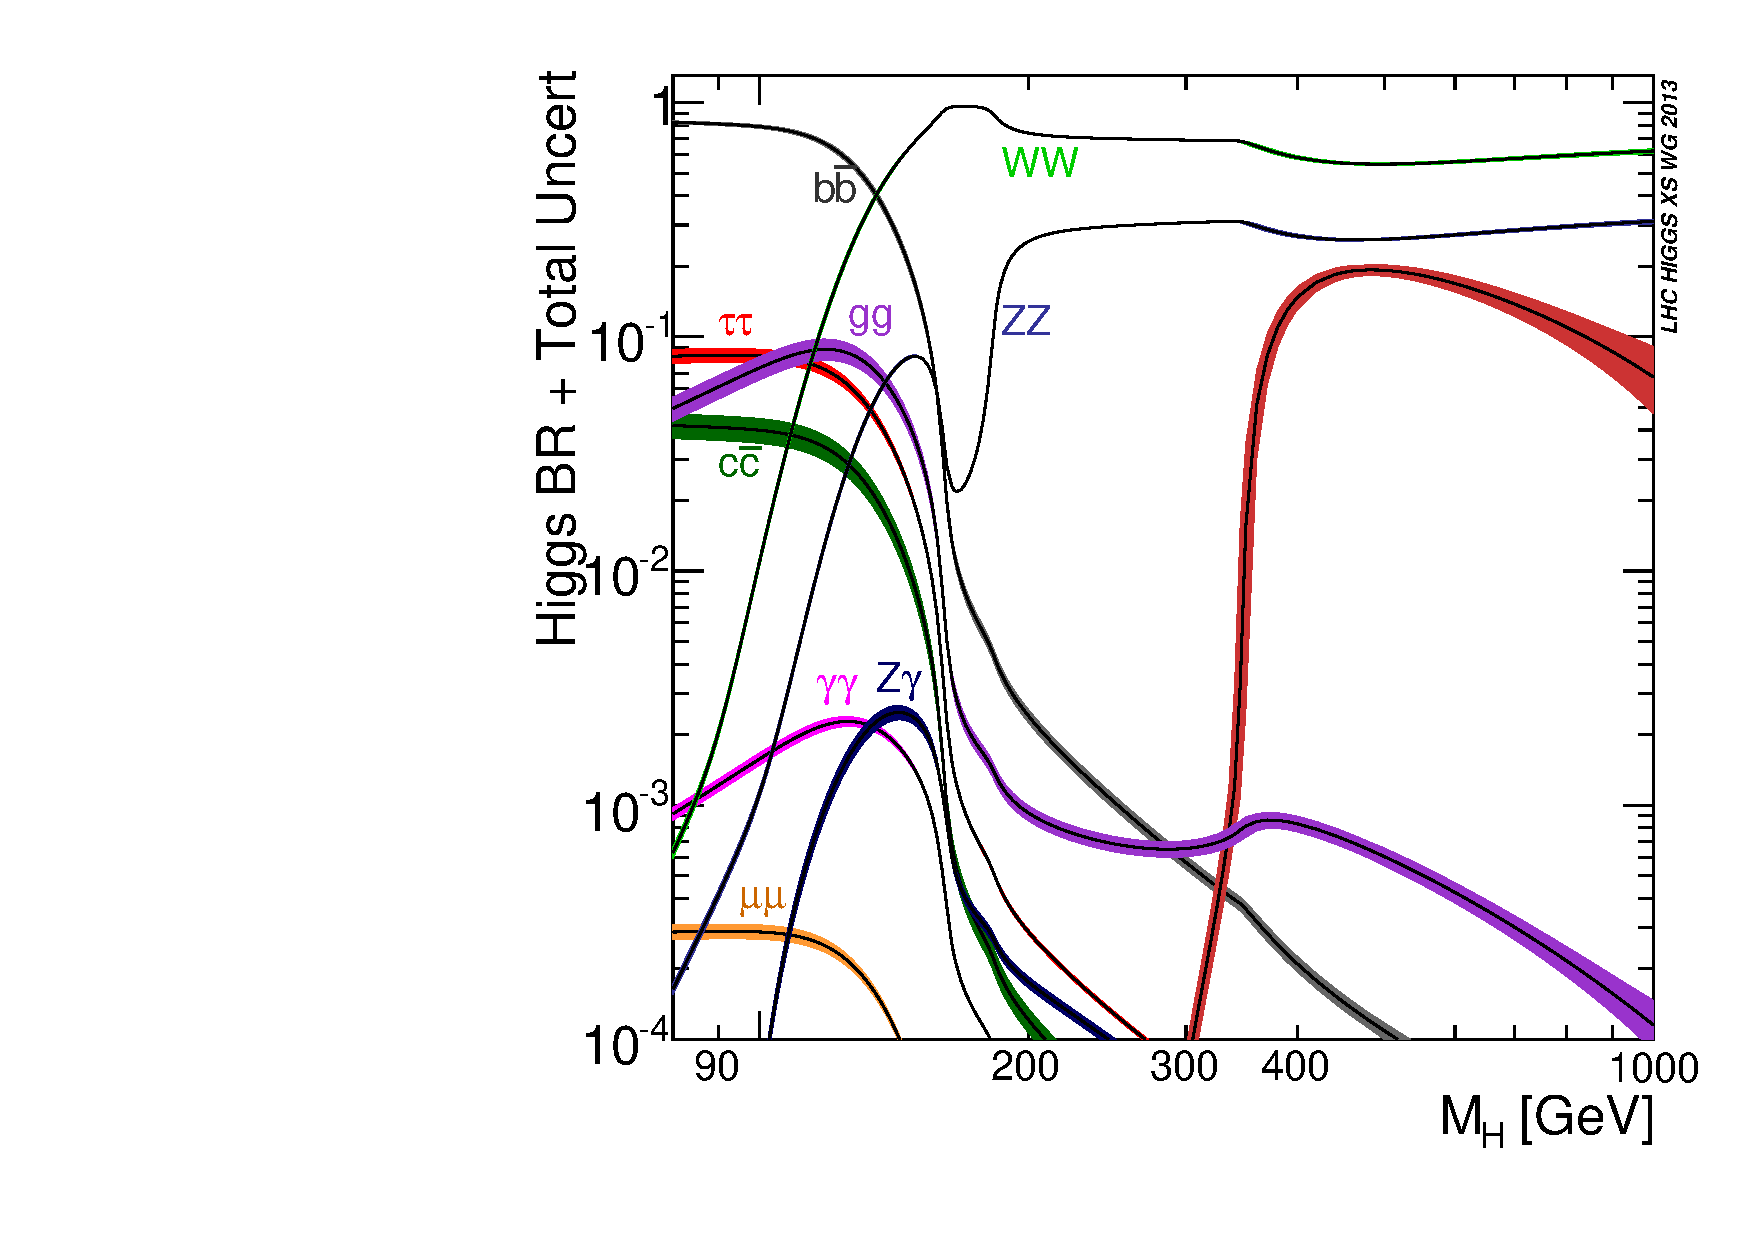
\includegraphics[width=0.75\textwidth]{plots/Higgs_BR.pdf}
        \end{figure}
    \end{column}
    \begin{column}{0.49\textwidth}
		\begin{figure}[t]
        \centering \textcolor{color1}{Special case: $H \rightarrow \gamma\gamma$}\\
        \vspace{0.5cm}
        \centering \begin{tikzpicture}[line width=1.5pt, scale=1.2]
\draw[step=0.5cm, very thin, transparent] (0cm,0cm) grid (4cm,2cm);

\draw[scalarnoarrow, color1, line width=3pt] (0cm,1cm) -- (1.5cm,1cm);
\node at (0cm-0.3cm,1cm) [color1]{H};

\draw[fermion] (1.5cm,1cm) -- (2.5cm,0cm);
\draw[fermion] (2.5cm,2cm) -- (1.5cm,1cm);
\draw[fermion] (2.5cm,0cm) -- node[left]{$t$} (2.5cm,2cm);

\draw[vector] (2.5cm,0cm) -- (4cm,0cm);
\node at (4cm+0.2cm,0cm) {$\gamma$};

\draw[vector] (2.5cm,2cm) -- (4cm,2cm);
\node at (4cm+0.2cm,2cm) {$\gamma$};

\end{tikzpicture}

        \end{figure}
    \end{column}
    \end{columns}
    \begin{minipage}{1.\textwidth}
		\begin{center}
		\begin{table}[c]
        \centering
        \hspace*{-0.5cm}
        \begin{tabular}{l|l|l}
        Decay Channel                     & Branching Fraction & Characteristics      \\ \hline \hline
        $H \rightarrow b\overline{b}$     & $58.4\%$           & High QCD             \\ \hline
        $H \rightarrow W^+W^-$            & $21.4\%$           & Jets + MET           \\ \hline
        $H \rightarrow \tau^+ \tau^-$     & $6.27\%$           & Jets + MET		      \\ \hline
        $H \rightarrow ZZ \rightarrow 4l$ & $2.62\%$           & High mass resolution \\ \hline
        $H \rightarrow \gamma \gamma$     & $0.227\%$          & High mass resolution \\
        \end{tabular}
        \end{table}
		\end{center}
    \end{minipage}
\end{frame}

\begin{frame}
    \frametitle{July 2012: Higgs Discovery @ CMS $\&$ ATLAS}
	\begin{columns}
    \begin{column}{0.49\textwidth}
        \begin{figure}[t]
			\\
			\vspace{-0.5cm}
			\centering \textcolor{color1}{$H \rightarrow \gamma\gamma$}\\
            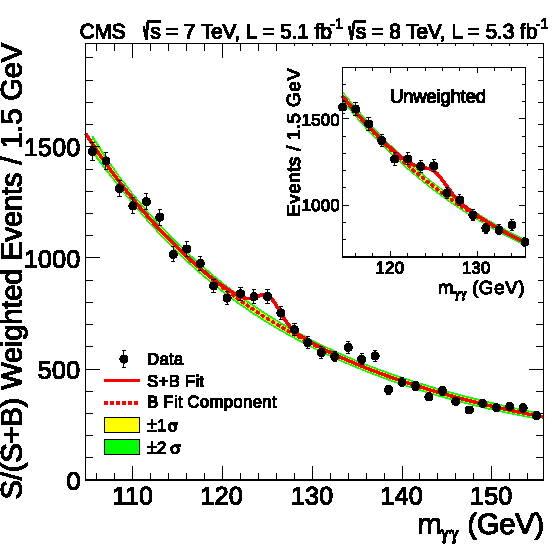
\includegraphics[width=0.75\textwidth]{plots/higgsGG_discovery.pdf}
        \end{figure}\\
		\vspace{-0.9cm}
		\begin{figure}[t]
			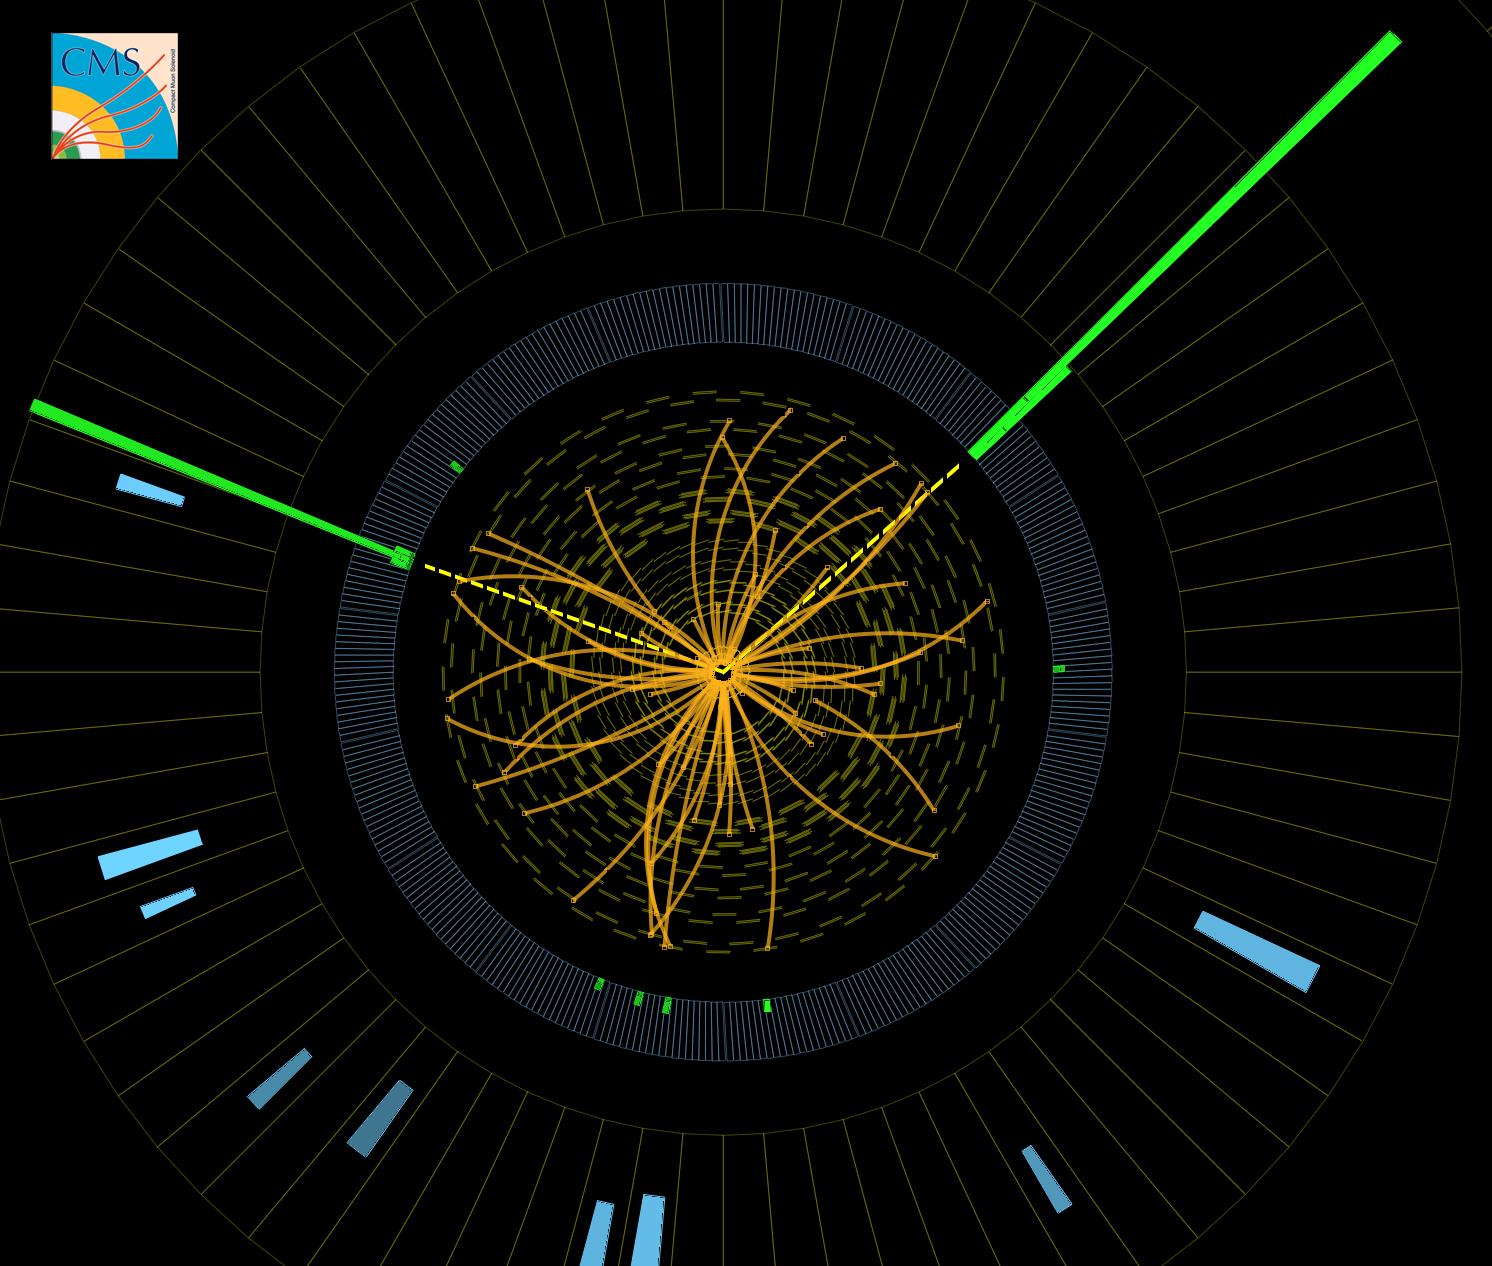
\includegraphics[width=0.7\textwidth]{plots/cms_event_display.png}
        \end{figure}
    \end{column}
	\begin{column}{0.49\textwidth}
        \begin{figure}[t]
			\\
			\vspace{-0.5cm}
			\centering \textcolor{color1}{$H \rightarrow ZZ \rightarrow 4l$}\\
            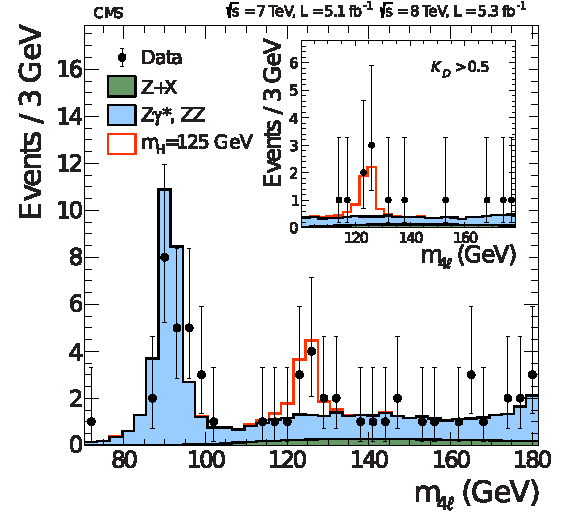
\includegraphics[width=0.8\textwidth]{plots/higgsZZ_discovery.pdf}
        \end{figure}\\
		\vspace{-0.9cm}
		\begin{figure}[t]
			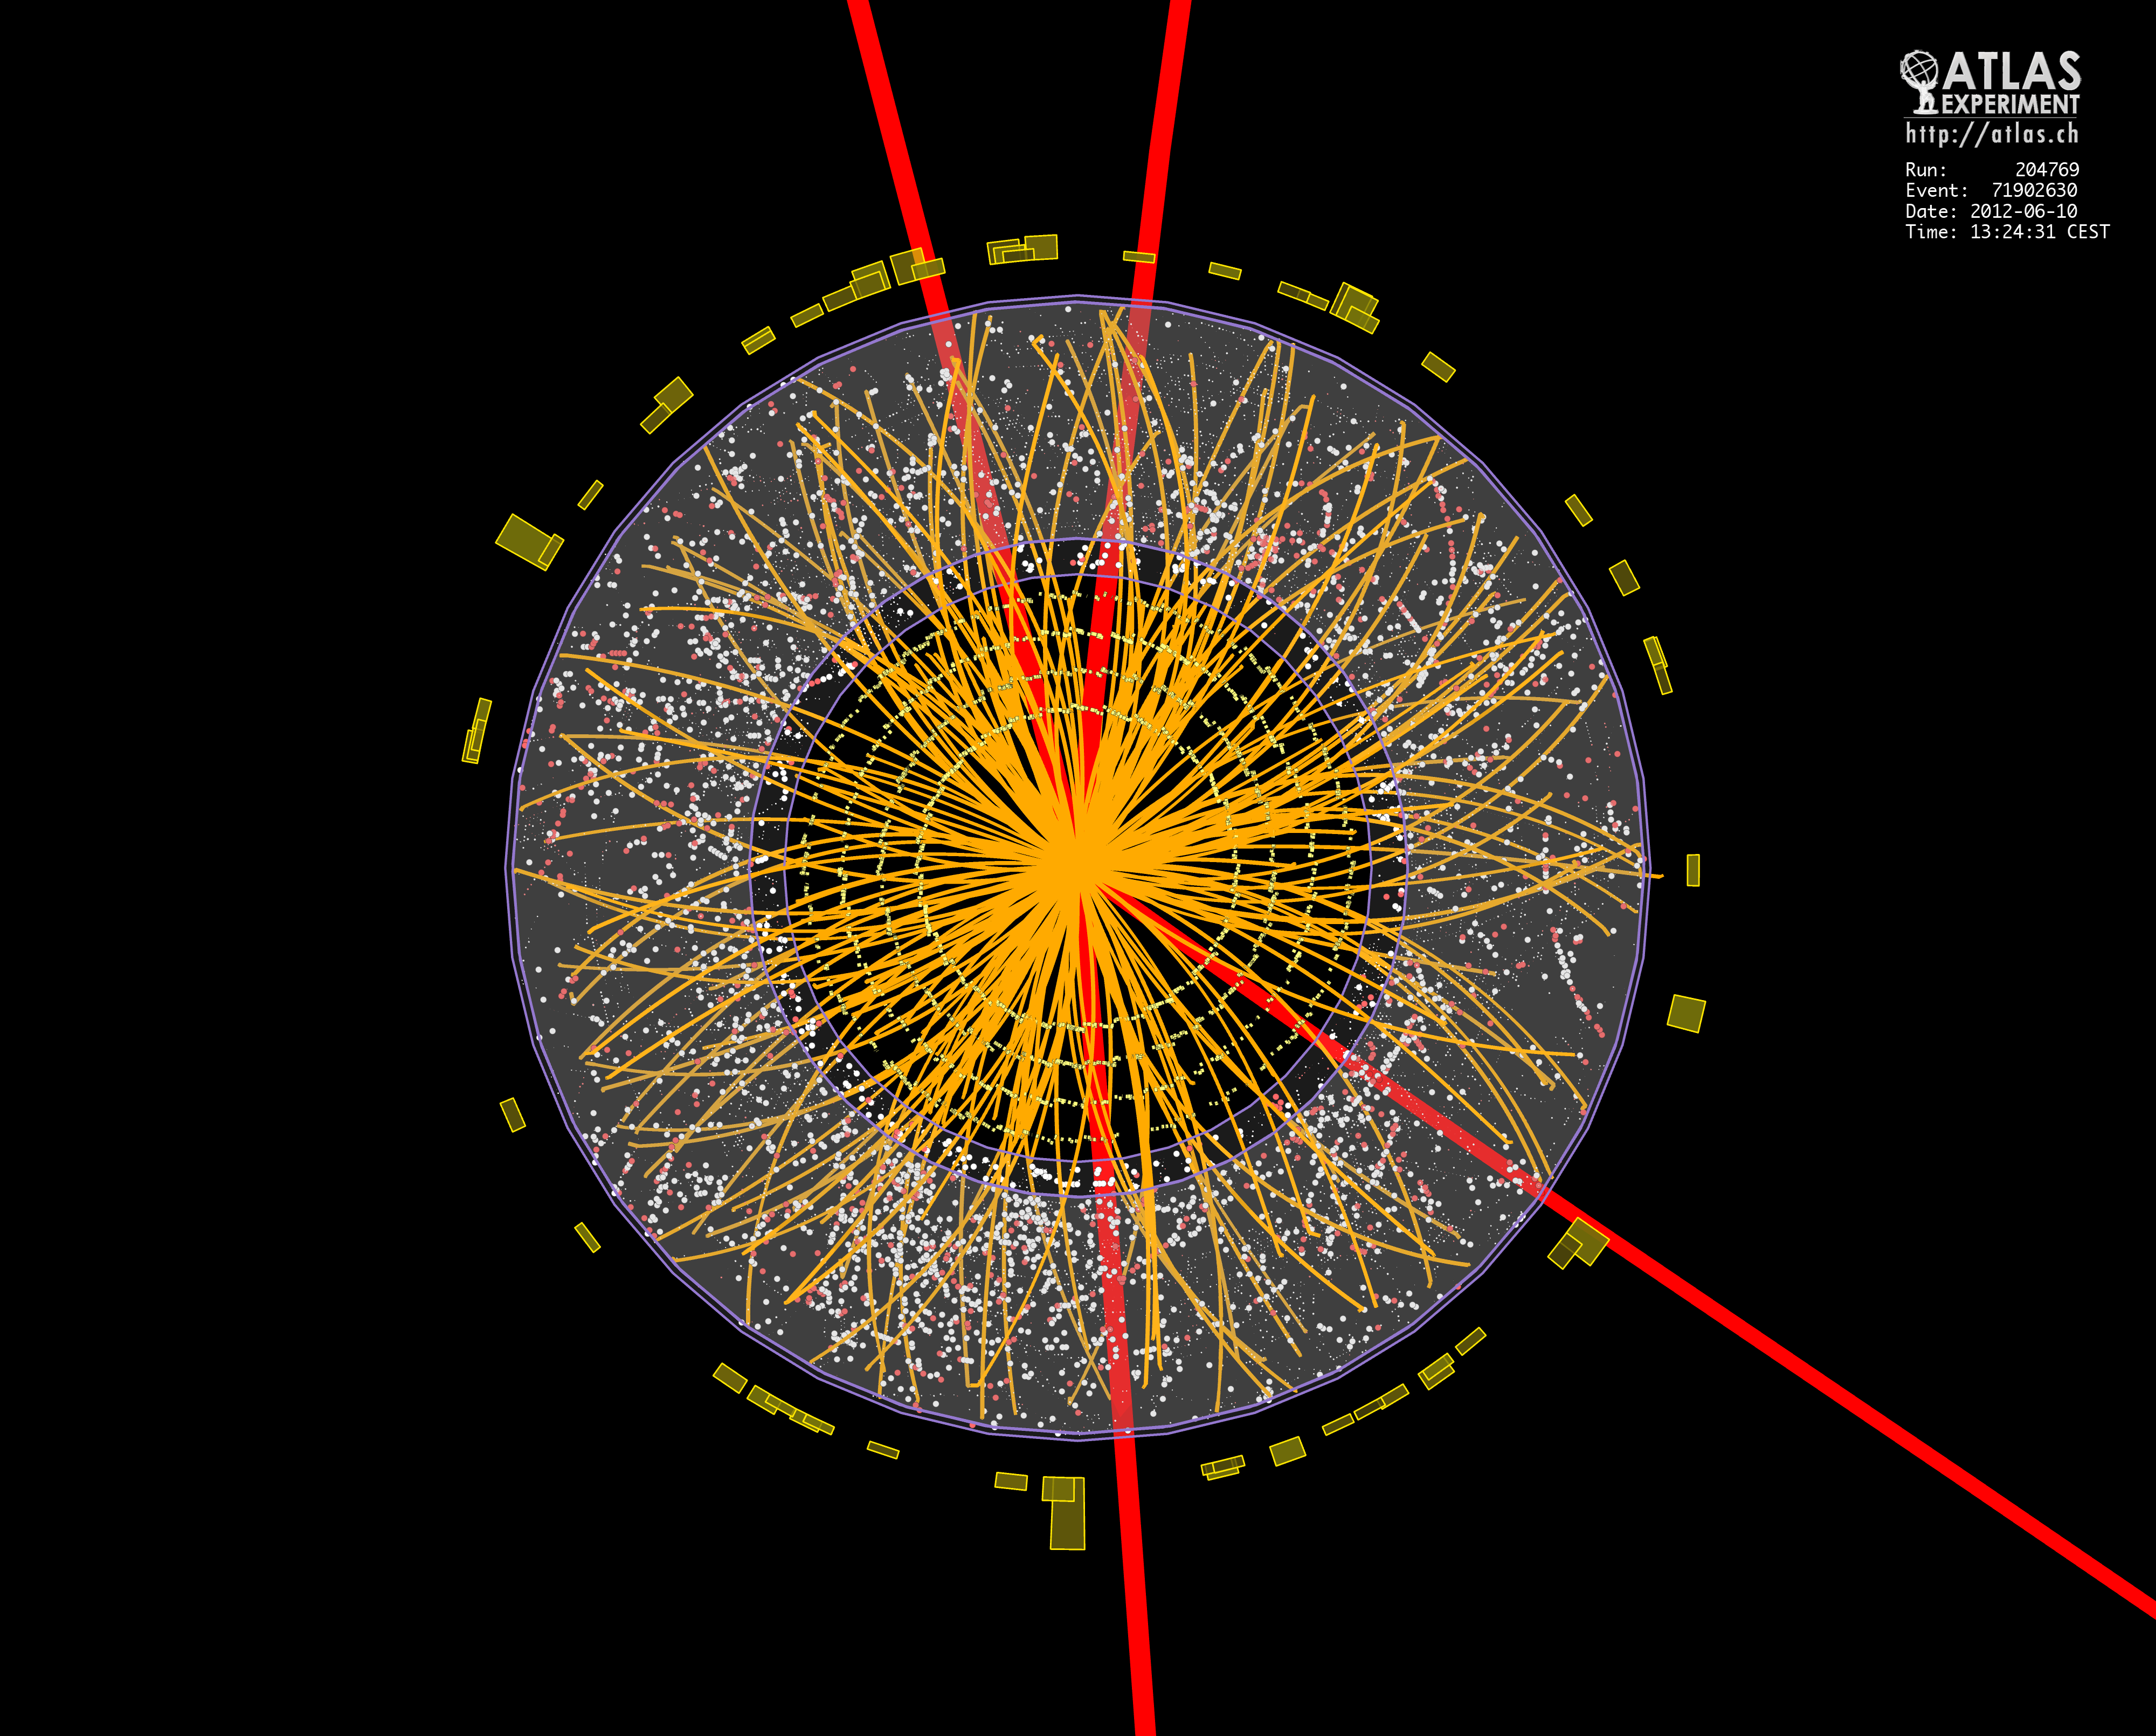
\includegraphics[width=0.7\textwidth]{plots/atlas_event_display.png}
        \end{figure}
    \end{column}
	\end{columns}
\end{frame}

\begin{frame}
	\frametitle{July 2012: Higgs Discovery @ CMS $\&$ ATLAS}
	\begin{columns}
	\begin{column}{0.49\textwidth}
		\begin{itemize}
			\item CMS-HIG-12-028:
			\begin{itemize}
				\item \textcolor{color1}{$5.0\sigma$}: $ 125.3 \pm 0.4 \,\text{(stat)} \pm 0.5 \,\text{(sys)}\, \text{GeV}$
			\end{itemize}
			\item CERN-PH-EP-2012-218:
			\begin{itemize}
				\item \textcolor{color1}{$5.9\sigma$}: $ 126.0 \pm 0.4 \, \text{(stat)} \pm 0.4 \, \text{(sys)}\, \text{GeV}$
			\end{itemize}
		\end{itemize}
		\begin{figure}[t]
			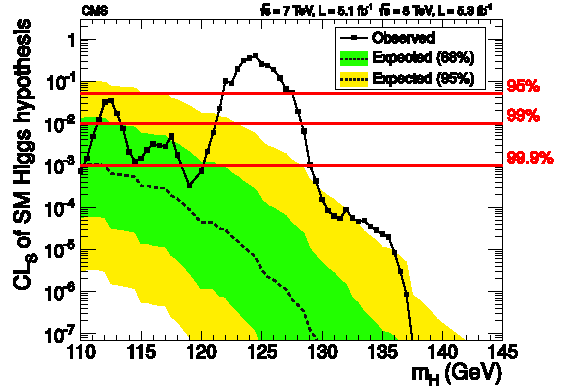
\includegraphics[width=1.\textwidth]{plots/higgs_combined_cls.pdf}
		\end{figure}
	\end{column}
	\begin{column}{0.49\textwidth}
		\begin{figure}[t]
			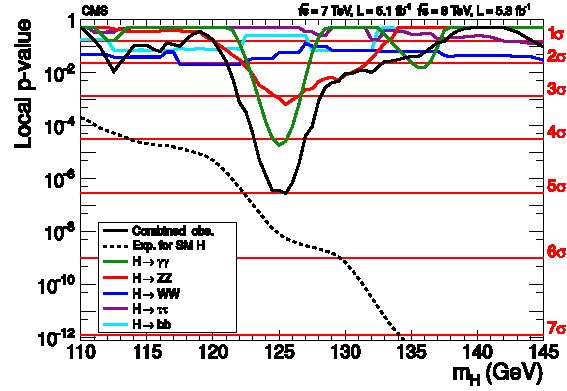
\includegraphics[width=1.\textwidth]{plots/higgs_p_value.pdf}
		\end{figure}
		\begin{figure}[t]
			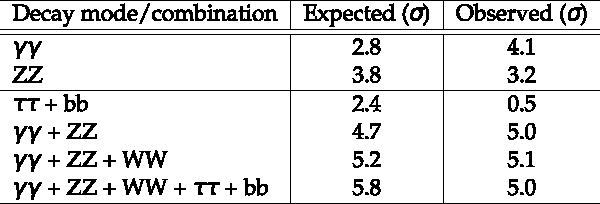
\includegraphics[width=1.\textwidth]{plots/higgs_pvalue_table.pdf}
		\end{figure}
	\end{column}
	\end{columns}
\end{frame}

\begin{frame}
	\frametitle{The Next Generation: $13\,\text{TeV}$ $\&$ More Data...}
	\begin{columns}
	\begin{column}{0.49\textwidth}
		\begin{figure}[t]
			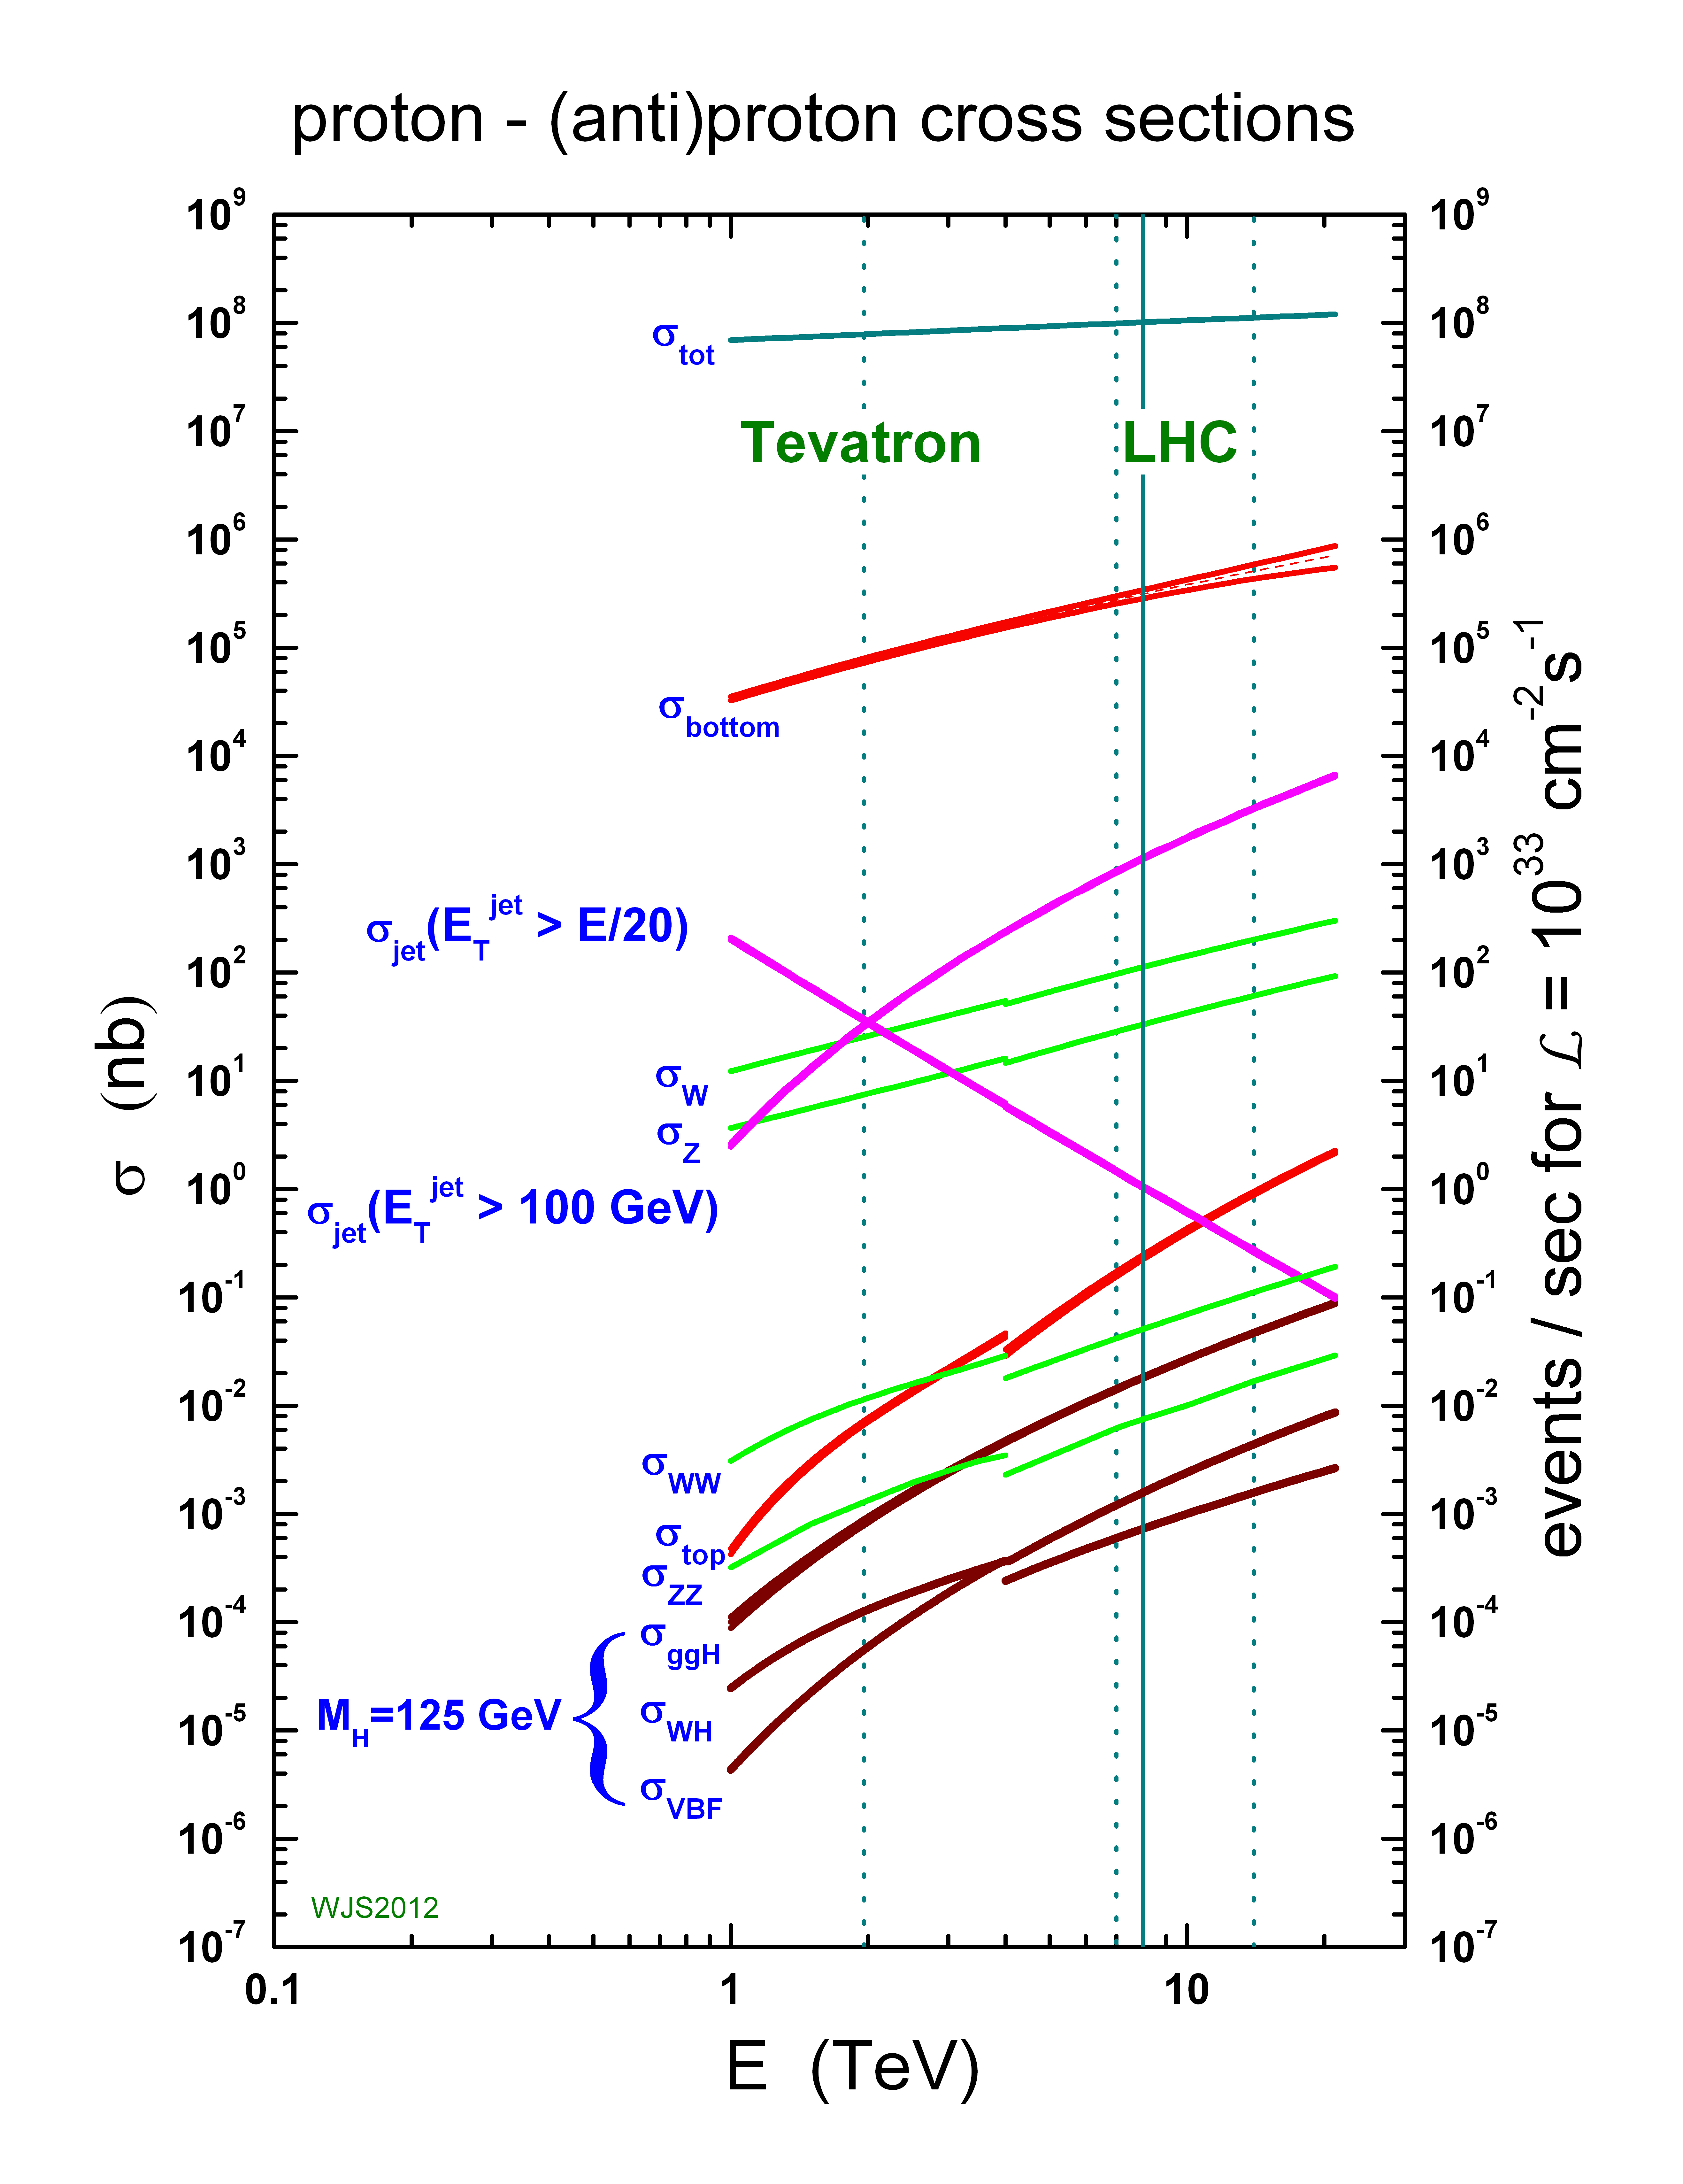
\includegraphics[width=1.\textwidth]{plots/crosssections2013.jpg}
		\end{figure}
	\end{column}
	\begin{column}{0.49\textwidth}
		\begin{figure}[t]
			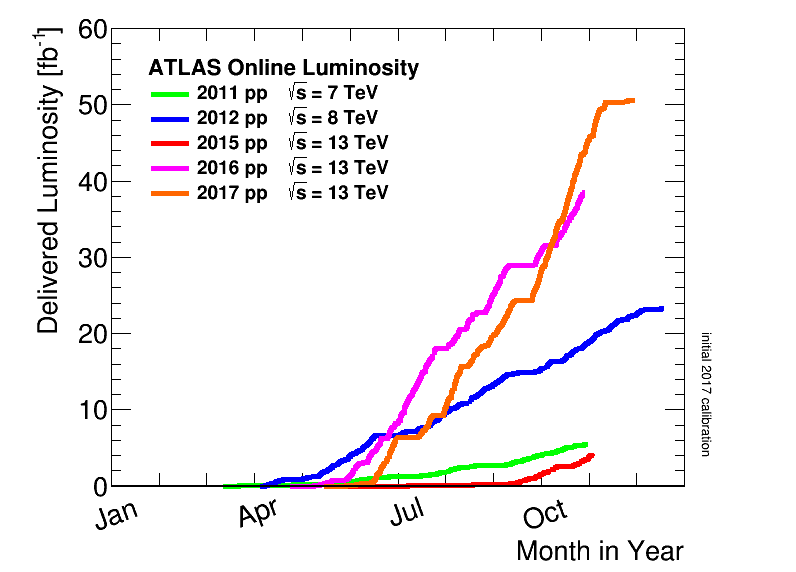
\includegraphics[width=1.\textwidth]{plots/intlumivsyear.png}
		\end{figure}
		\begin{itemize}
			\item More integrated luminosity (higher statistics)
			\item Higher cross sections for interesting physics
		\end{itemize}
	\end{column}
	\end{columns}
\end{frame}

\begin{frame}
	\frametitle{Return of the Higgs Boson}
	PLACEHOLDER: HIG-18-001
\end{frame}

\begin{frame}
	\frametitle{HL-LHC - The Final Frontier?}
	PLACEHOLDER: HL Upgrade
\end{frame}

\begin{frame}
	\frametitle{Exciting Times Ahead...}
	\begin{columns}
	\begin{column}{0.49\textwidth}
	\begin{itemize}
		\item Higgs boson as a probe for new physics
		\item Measurement of CP properties
		\item Discovery in missing decay channels
		\item More Higgs bosons? (2HDM)
		\item ILC: Higgs factory
		\item Stay tuned!!!
	\end{itemize}
  \end{column}
  \begin{column}{0.49\textwidth}
	\begin{figure}[t]
		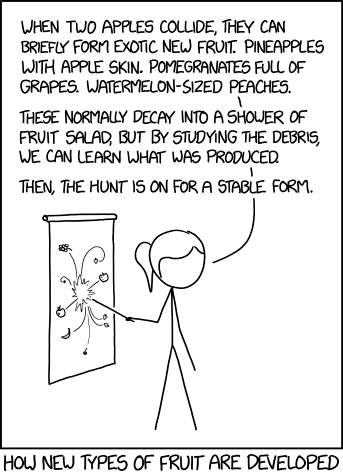
\includegraphics[width=0.75\textwidth]{plots/fruit_collider.png}
	\end{figure}
  \end{column}
\end{columns}
	\\
	\centering \textcolor{color1}{http://phdcomics.com/comics.php?f=1489}
\end{frame}
\end{document}
